\begin{tikzpicture}[node distance=6mm and 10mm]
  % every frame
  \fcard{g}{sbblue}{\faCamera}{Grab 1080p frame, measure $\Delta t$}{}
  \fdec{b}{sbblue}{Blocked for 3\,s?}{below=of g}
  \fcard{bb}{sbred}{\faVolumeUp}{Voice: camera blocked, pause, log}{left=of b}
  \fcard{c}{sbblue}{\faCrop}{640$\times$640 crop}{below=of b}
  \fcard{y}{sbblue}{\faProjectDiagram}{\gls{yolo}11n on the \gls{npu}}{below=of c}
  \fcard{e}{sbblue}{\faFilter}{Max score per class, \gls{ema} update}{below=of y}
  % decision
  \fdec{d1}{sbred}{Above cutoff?}{right=26mm of g}
  \fdec{d2}{sbred}{Held for confirm time?}{below=of d1}
  \fdec{d3}{sbred}{In cool-down?}{below=of d2}
  \fcard{t}{sbred}{\faLayerGroup}{Select tier from duration and recent events}{below=of d3}
  \fcard{a}{sbred}{\faBell}{Light pattern and explained voice message}{below=of t}
  \fcard{l}{sbblue}{\faDatabase}{Write event to SQLite}{below=of a}

  \coordinate (top) at ($(g.north)+(0,14mm)$);
  \coordinate (lane) at ($(d1.east)+(9mm,0)$);
  \draw[farr] (g) -- (b);
  \draw[farr] (b) -- node[flab, right]{no} (c);
  \draw[farr] (b) -- node[flab, above]{yes} (bb);
  \draw[farr] (bb.north) |- (g.west);
  \draw[farr] (c) -- (y); \draw[farr] (y) -- (e);
  \draw[farr] (e.east) -- ++(8mm,0) |- (d1.west);
  \draw[farr] (d1) -- node[flab, right]{yes} (d2);
  \draw[farr] (d2) -- node[flab, right]{yes} (d3);
  \draw[farr] (d3) -- node[flab, right]{no} (t);
  \draw[farr] (t) -- (a); \draw[farr] (a) -- (l);
  % return lane to the next frame
  \draw[fline] (d1.east) -- node[flab, above]{no} (d1.east -| lane);
  \draw[fline] (d2.east) -- node[flab, above]{no} (d2.east -| lane);
  \draw[fline] (d3.east) -- node[flab, above]{yes} (d3.east -| lane);
  \draw[fline] (l.east) -- (l.east -| lane);
  \draw[farr] (l.east -| lane) -- (lane |- top) -- node[flab, above, pos=0.5]{next frame} (top) -- (g.north);

  % letters tie the steps to the worked example below
  \linknum{e.north west}{}{A}
  \linknum{d1.west}{}{B}
  \linknum{d2.west}{}{C}
  \linknum{a.north west}{}{D}

  % worked example: one yawn, frame by frame
  \begin{scope}[shift={($(bb.west |- l.south)+(30mm,-37mm)$)}, font=\small]
    \node[inner sep=0, anchor=south west] at (0.030,0.950) {
\includegraphics[width=1.940cm,height=1.940cm]{Figures/guide_0.png}};
\node[inner sep=0, anchor=south west] at (2.030,0.950) {
\includegraphics[width=1.940cm,height=1.940cm]{Figures/guide_0.png}};
\node[inner sep=0, anchor=south west] at (4.030,0.950) {
\includegraphics[width=1.940cm,height=1.940cm]{Figures/guide_0.png}};
\node[inner sep=0, anchor=south west] at (6.030,0.950) {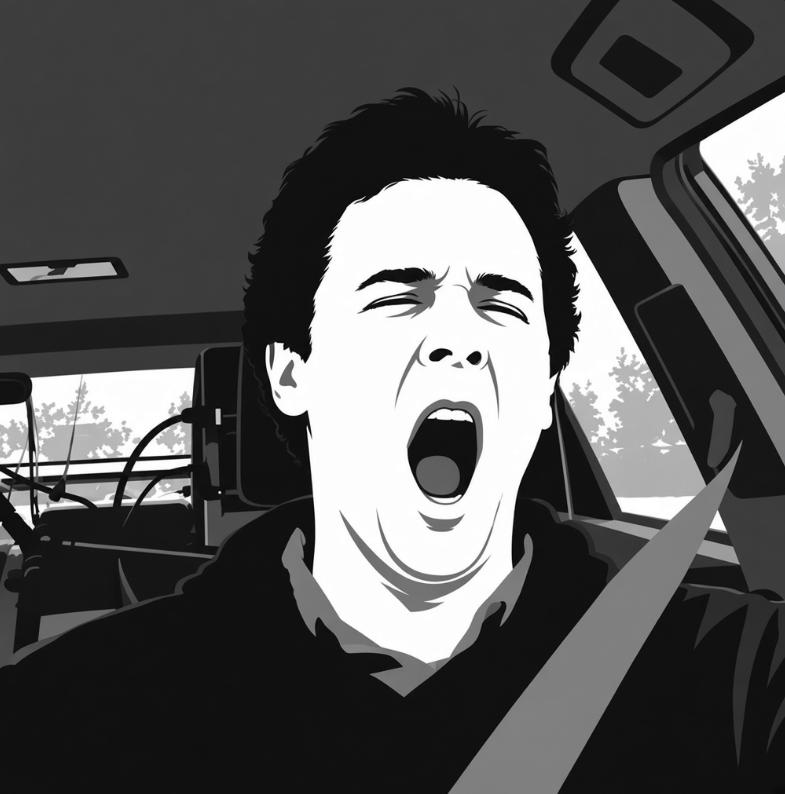
\includegraphics[width=1.940cm,height=1.940cm]{Figures/guide_2.png}};
\node[inner sep=0, anchor=south west] at (8.030,0.950) {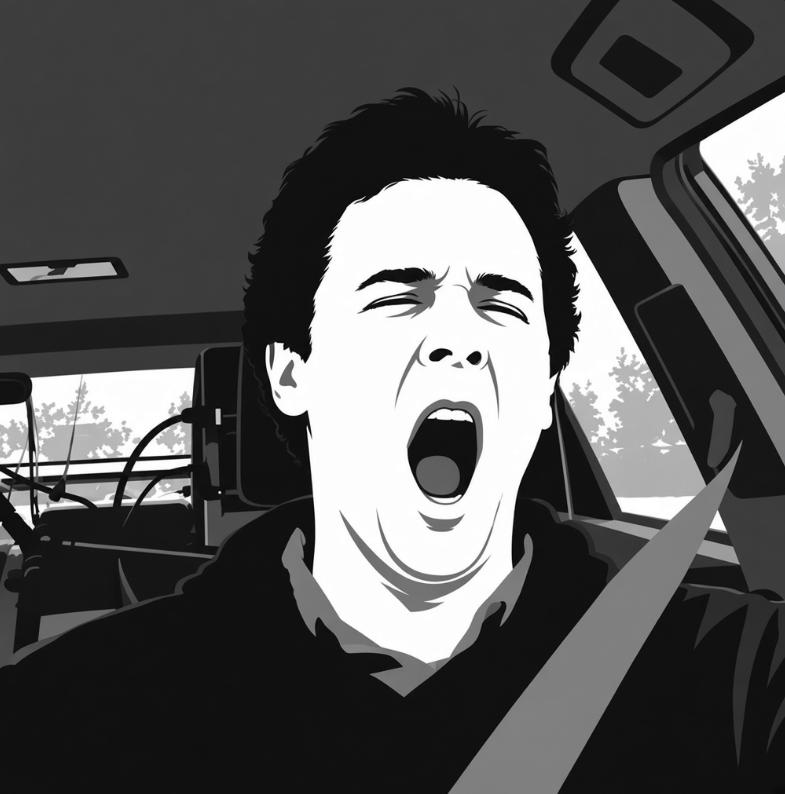
\includegraphics[width=1.940cm,height=1.940cm]{Figures/guide_2.png}};
\node[inner sep=0, anchor=south west] at (10.030,0.950) {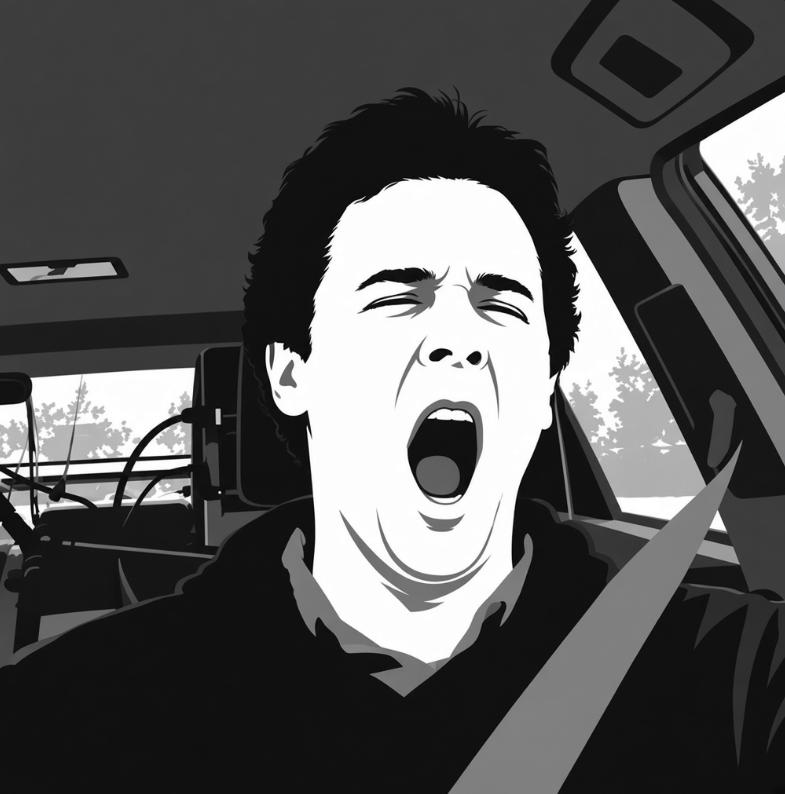
\includegraphics[width=1.940cm,height=1.940cm]{Figures/guide_2.png}};
\node[inner sep=0, anchor=south west] at (12.030,0.950) {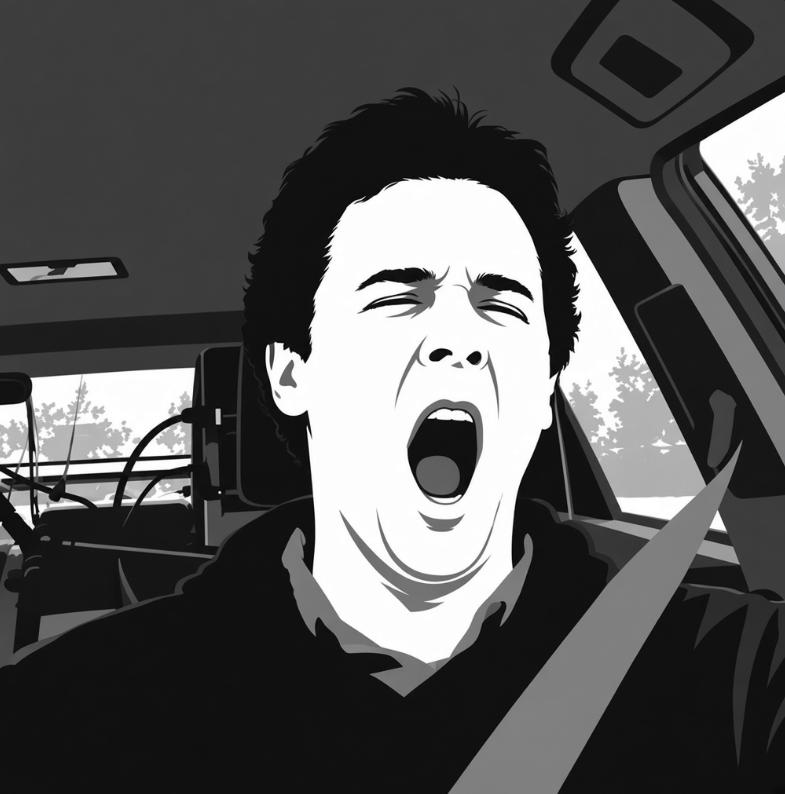
\includegraphics[width=1.940cm,height=1.940cm]{Figures/guide_2.png}};
\node[inner sep=0, anchor=south west] at (14.030,0.950) {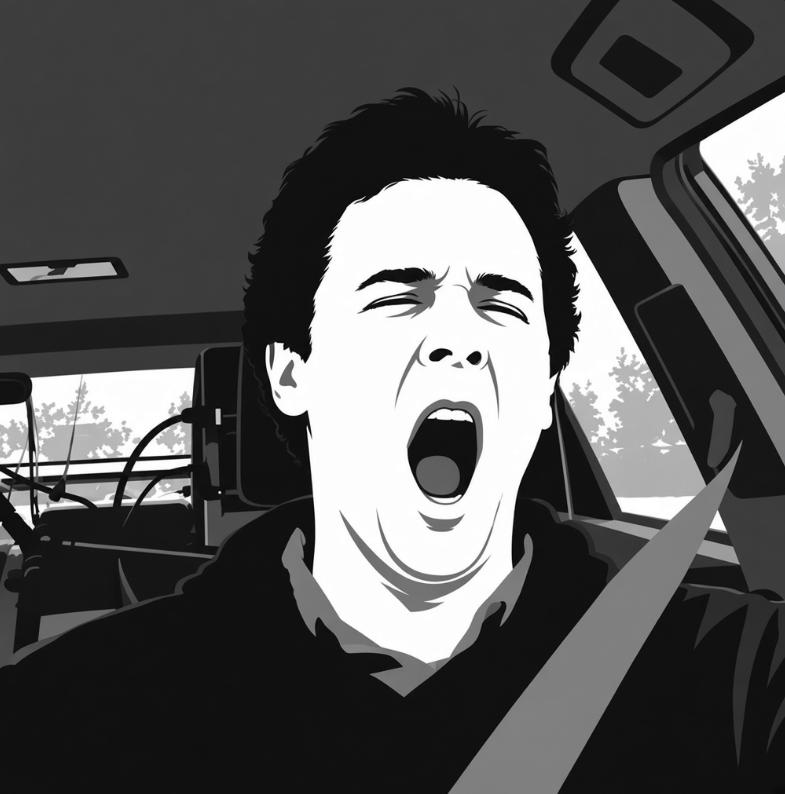
\includegraphics[width=1.940cm,height=1.940cm]{Figures/guide_2.png}};
\node[anchor=east] at (-0.15,1.950) {Frames};
\node[anchor=east] at (-0.15,0.210) {Raw score $x_t$};
\node[anchor=east] at (-0.15,-0.510) {Smoothed $s_t$};
\node[anchor=east] at (-0.15,-1.230) {$s_t > \theta$};
\filldraw[draw=white, line width=0.6pt, fill=sbblue!6!white] (0.000,0.000) rectangle ++(0.400,0.420);
\filldraw[draw=white, line width=0.6pt, fill=sbblue!1!white] (0.000,-0.720) rectangle ++(0.400,0.420);
\filldraw[draw=white, line width=0.6pt, fill=gray!12] (0.000,-1.440) rectangle ++(0.400,0.420);
\filldraw[draw=white, line width=0.6pt, fill=sbblue!7!white] (0.400,0.000) rectangle ++(0.400,0.420);
\filldraw[draw=white, line width=0.6pt, fill=sbblue!2!white] (0.400,-0.720) rectangle ++(0.400,0.420);
\filldraw[draw=white, line width=0.6pt, fill=gray!12] (0.400,-1.440) rectangle ++(0.400,0.420);
\filldraw[draw=white, line width=0.6pt, fill=sbblue!5!white] (0.800,0.000) rectangle ++(0.400,0.420);
\filldraw[draw=white, line width=0.6pt, fill=sbblue!2!white] (0.800,-0.720) rectangle ++(0.400,0.420);
\filldraw[draw=white, line width=0.6pt, fill=gray!12] (0.800,-1.440) rectangle ++(0.400,0.420);
\filldraw[draw=white, line width=0.6pt, fill=sbblue!3!white] (1.200,0.000) rectangle ++(0.400,0.420);
\filldraw[draw=white, line width=0.6pt, fill=sbblue!3!white] (1.200,-0.720) rectangle ++(0.400,0.420);
\filldraw[draw=white, line width=0.6pt, fill=gray!12] (1.200,-1.440) rectangle ++(0.400,0.420);
\filldraw[draw=white, line width=0.6pt, fill=sbblue!92!white] (1.600,0.000) rectangle ++(0.400,0.420);
\filldraw[draw=white, line width=0.6pt, fill=sbblue!16!white] (1.600,-0.720) rectangle ++(0.400,0.420);
\filldraw[draw=white, line width=0.6pt, fill=gray!12] (1.600,-1.440) rectangle ++(0.400,0.420);
\filldraw[draw=white, line width=0.6pt, fill=sbblue!3!white] (2.000,0.000) rectangle ++(0.400,0.420);
\filldraw[draw=white, line width=0.6pt, fill=sbblue!14!white] (2.000,-0.720) rectangle ++(0.400,0.420);
\filldraw[draw=white, line width=0.6pt, fill=gray!12] (2.000,-1.440) rectangle ++(0.400,0.420);
\filldraw[draw=white, line width=0.6pt, fill=sbblue!6!white] (2.400,0.000) rectangle ++(0.400,0.420);
\filldraw[draw=white, line width=0.6pt, fill=sbblue!13!white] (2.400,-0.720) rectangle ++(0.400,0.420);
\filldraw[draw=white, line width=0.6pt, fill=gray!12] (2.400,-1.440) rectangle ++(0.400,0.420);
\filldraw[draw=white, line width=0.6pt, fill=sbblue!10!white] (2.800,0.000) rectangle ++(0.400,0.420);
\filldraw[draw=white, line width=0.6pt, fill=sbblue!13!white] (2.800,-0.720) rectangle ++(0.400,0.420);
\filldraw[draw=white, line width=0.6pt, fill=gray!12] (2.800,-1.440) rectangle ++(0.400,0.420);
\filldraw[draw=white, line width=0.6pt, fill=sbblue!88!white] (3.200,0.000) rectangle ++(0.400,0.420);
\filldraw[draw=white, line width=0.6pt, fill=sbblue!24!white] (3.200,-0.720) rectangle ++(0.400,0.420);
\filldraw[draw=white, line width=0.6pt, fill=gray!12] (3.200,-1.440) rectangle ++(0.400,0.420);
\filldraw[draw=white, line width=0.6pt, fill=sbblue!4!white] (3.600,0.000) rectangle ++(0.400,0.420);
\filldraw[draw=white, line width=0.6pt, fill=sbblue!21!white] (3.600,-0.720) rectangle ++(0.400,0.420);
\filldraw[draw=white, line width=0.6pt, fill=gray!12] (3.600,-1.440) rectangle ++(0.400,0.420);
\filldraw[draw=white, line width=0.6pt, fill=sbblue!7!white] (4.000,0.000) rectangle ++(0.400,0.420);
\filldraw[draw=white, line width=0.6pt, fill=sbblue!19!white] (4.000,-0.720) rectangle ++(0.400,0.420);
\filldraw[draw=white, line width=0.6pt, fill=gray!12] (4.000,-1.440) rectangle ++(0.400,0.420);
\filldraw[draw=white, line width=0.6pt, fill=sbblue!7!white] (4.400,0.000) rectangle ++(0.400,0.420);
\filldraw[draw=white, line width=0.6pt, fill=sbblue!17!white] (4.400,-0.720) rectangle ++(0.400,0.420);
\filldraw[draw=white, line width=0.6pt, fill=gray!12] (4.400,-1.440) rectangle ++(0.400,0.420);
\filldraw[draw=white, line width=0.6pt, fill=sbblue!6!white] (4.800,0.000) rectangle ++(0.400,0.420);
\filldraw[draw=white, line width=0.6pt, fill=sbblue!15!white] (4.800,-0.720) rectangle ++(0.400,0.420);
\filldraw[draw=white, line width=0.6pt, fill=gray!12] (4.800,-1.440) rectangle ++(0.400,0.420);
\filldraw[draw=white, line width=0.6pt, fill=sbblue!3!white] (5.200,0.000) rectangle ++(0.400,0.420);
\filldraw[draw=white, line width=0.6pt, fill=sbblue!14!white] (5.200,-0.720) rectangle ++(0.400,0.420);
\filldraw[draw=white, line width=0.6pt, fill=gray!12] (5.200,-1.440) rectangle ++(0.400,0.420);
\filldraw[draw=white, line width=0.6pt, fill=sbblue!6!white] (5.600,0.000) rectangle ++(0.400,0.420);
\filldraw[draw=white, line width=0.6pt, fill=sbblue!12!white] (5.600,-0.720) rectangle ++(0.400,0.420);
\filldraw[draw=white, line width=0.6pt, fill=gray!12] (5.600,-1.440) rectangle ++(0.400,0.420);
\filldraw[draw=white, line width=0.6pt, fill=sbblue!86!white] (6.000,0.000) rectangle ++(0.400,0.420);
\filldraw[draw=white, line width=0.6pt, fill=sbblue!24!white] (6.000,-0.720) rectangle ++(0.400,0.420);
\filldraw[draw=white, line width=0.6pt, fill=gray!12] (6.000,-1.440) rectangle ++(0.400,0.420);
\filldraw[draw=white, line width=0.6pt, fill=sbblue!90!white] (6.400,0.000) rectangle ++(0.400,0.420);
\filldraw[draw=white, line width=0.6pt, fill=sbblue!34!white] (6.400,-0.720) rectangle ++(0.400,0.420);
\filldraw[draw=white, line width=0.6pt, fill=gray!12] (6.400,-1.440) rectangle ++(0.400,0.420);
\filldraw[draw=white, line width=0.6pt, fill=sbblue!84!white] (6.800,0.000) rectangle ++(0.400,0.420);
\filldraw[draw=white, line width=0.6pt, fill=sbblue!41!white] (6.800,-0.720) rectangle ++(0.400,0.420);
\filldraw[draw=white, line width=0.6pt, fill=gray!12] (6.800,-1.440) rectangle ++(0.400,0.420);
\filldraw[draw=white, line width=0.6pt, fill=sbblue!86!white] (7.200,0.000) rectangle ++(0.400,0.420);
\filldraw[draw=white, line width=0.6pt, fill=sbblue!48!white] (7.200,-0.720) rectangle ++(0.400,0.420);
\filldraw[draw=white, line width=0.6pt, fill=gray!12] (7.200,-1.440) rectangle ++(0.400,0.420);
\filldraw[draw=white, line width=0.6pt, fill=sbblue!86!white] (7.600,0.000) rectangle ++(0.400,0.420);
\filldraw[draw=white, line width=0.6pt, fill=sbblue!54!white] (7.600,-0.720) rectangle ++(0.400,0.420);
\filldraw[draw=white, line width=0.6pt, fill=sbgold!85] (7.600,-1.440) rectangle ++(0.400,0.420);
\filldraw[draw=white, line width=0.6pt, fill=sbblue!86!white] (8.000,0.000) rectangle ++(0.400,0.420);
\filldraw[draw=white, line width=0.6pt, fill=sbblue!59!white] (8.000,-0.720) rectangle ++(0.400,0.420);
\filldraw[draw=white, line width=0.6pt, fill=sbgold!85] (8.000,-1.440) rectangle ++(0.400,0.420);
\filldraw[draw=white, line width=0.6pt, fill=sbblue!81!white] (8.400,0.000) rectangle ++(0.400,0.420);
\filldraw[draw=white, line width=0.6pt, fill=sbblue!62!white] (8.400,-0.720) rectangle ++(0.400,0.420);
\filldraw[draw=white, line width=0.6pt, fill=sbgold!85] (8.400,-1.440) rectangle ++(0.400,0.420);
\filldraw[draw=white, line width=0.6pt, fill=sbblue!86!white] (8.800,0.000) rectangle ++(0.400,0.420);
\filldraw[draw=white, line width=0.6pt, fill=sbblue!66!white] (8.800,-0.720) rectangle ++(0.400,0.420);
\filldraw[draw=white, line width=0.6pt, fill=sbgold!85] (8.800,-1.440) rectangle ++(0.400,0.420);
\filldraw[draw=white, line width=0.6pt, fill=sbblue!91!white] (9.200,0.000) rectangle ++(0.400,0.420);
\filldraw[draw=white, line width=0.6pt, fill=sbblue!70!white] (9.200,-0.720) rectangle ++(0.400,0.420);
\filldraw[draw=white, line width=0.6pt, fill=sbgold!85] (9.200,-1.440) rectangle ++(0.400,0.420);
\filldraw[draw=white, line width=0.6pt, fill=sbblue!80!white] (9.600,0.000) rectangle ++(0.400,0.420);
\filldraw[draw=white, line width=0.6pt, fill=sbblue!71!white] (9.600,-0.720) rectangle ++(0.400,0.420);
\filldraw[draw=white, line width=0.6pt, fill=sbgold!85] (9.600,-1.440) rectangle ++(0.400,0.420);
\filldraw[draw=white, line width=0.6pt, fill=sbblue!89!white] (10.000,0.000) rectangle ++(0.400,0.420);
\filldraw[draw=white, line width=0.6pt, fill=sbblue!74!white] (10.000,-0.720) rectangle ++(0.400,0.420);
\filldraw[draw=white, line width=0.6pt, fill=sbgold!85] (10.000,-1.440) rectangle ++(0.400,0.420);
\filldraw[draw=white, line width=0.6pt, fill=sbblue!86!white] (10.400,0.000) rectangle ++(0.400,0.420);
\filldraw[draw=white, line width=0.6pt, fill=sbblue!76!white] (10.400,-0.720) rectangle ++(0.400,0.420);
\filldraw[draw=white, line width=0.6pt, fill=sbgold!85] (10.400,-1.440) rectangle ++(0.400,0.420);
\filldraw[draw=white, line width=0.6pt, fill=sbblue!83!white] (10.800,0.000) rectangle ++(0.400,0.420);
\filldraw[draw=white, line width=0.6pt, fill=sbblue!77!white] (10.800,-0.720) rectangle ++(0.400,0.420);
\filldraw[draw=white, line width=0.6pt, fill=sbgold!85] (10.800,-1.440) rectangle ++(0.400,0.420);
\filldraw[draw=white, line width=0.6pt, fill=sbblue!94!white] (11.200,0.000) rectangle ++(0.400,0.420);
\filldraw[draw=white, line width=0.6pt, fill=sbblue!80!white] (11.200,-0.720) rectangle ++(0.400,0.420);
\filldraw[draw=white, line width=0.6pt, fill=sbgold!85] (11.200,-1.440) rectangle ++(0.400,0.420);
\filldraw[draw=white, line width=0.6pt, fill=sbblue!89!white] (11.600,0.000) rectangle ++(0.400,0.420);
\filldraw[draw=white, line width=0.6pt, fill=sbblue!81!white] (11.600,-0.720) rectangle ++(0.400,0.420);
\filldraw[draw=white, line width=0.6pt, fill=sbred] (11.600,-1.440) rectangle ++(0.400,0.420);
\filldraw[draw=white, line width=0.6pt, fill=sbblue!81!white] (12.000,0.000) rectangle ++(0.400,0.420);
\filldraw[draw=white, line width=0.6pt, fill=sbblue!81!white] (12.000,-0.720) rectangle ++(0.400,0.420);
\filldraw[draw=white, line width=0.6pt, fill=sbgold!35] (12.000,-1.440) rectangle ++(0.400,0.420);
\filldraw[draw=white, line width=0.6pt, fill=sbblue!86!white] (12.400,0.000) rectangle ++(0.400,0.420);
\filldraw[draw=white, line width=0.6pt, fill=sbblue!82!white] (12.400,-0.720) rectangle ++(0.400,0.420);
\filldraw[draw=white, line width=0.6pt, fill=sbgold!35] (12.400,-1.440) rectangle ++(0.400,0.420);
\filldraw[draw=white, line width=0.6pt, fill=sbblue!88!white] (12.800,0.000) rectangle ++(0.400,0.420);
\filldraw[draw=white, line width=0.6pt, fill=sbblue!83!white] (12.800,-0.720) rectangle ++(0.400,0.420);
\filldraw[draw=white, line width=0.6pt, fill=sbgold!35] (12.800,-1.440) rectangle ++(0.400,0.420);
\filldraw[draw=white, line width=0.6pt, fill=sbblue!85!white] (13.200,0.000) rectangle ++(0.400,0.420);
\filldraw[draw=white, line width=0.6pt, fill=sbblue!83!white] (13.200,-0.720) rectangle ++(0.400,0.420);
\filldraw[draw=white, line width=0.6pt, fill=sbgold!35] (13.200,-1.440) rectangle ++(0.400,0.420);
\filldraw[draw=white, line width=0.6pt, fill=sbblue!89!white] (13.600,0.000) rectangle ++(0.400,0.420);
\filldraw[draw=white, line width=0.6pt, fill=sbblue!84!white] (13.600,-0.720) rectangle ++(0.400,0.420);
\filldraw[draw=white, line width=0.6pt, fill=sbgold!35] (13.600,-1.440) rectangle ++(0.400,0.420);
\filldraw[draw=white, line width=0.6pt, fill=sbblue!86!white] (14.000,0.000) rectangle ++(0.400,0.420);
\filldraw[draw=white, line width=0.6pt, fill=sbblue!84!white] (14.000,-0.720) rectangle ++(0.400,0.420);
\filldraw[draw=white, line width=0.6pt, fill=sbgold!35] (14.000,-1.440) rectangle ++(0.400,0.420);
\draw[gray!45, line width=0.4pt] (0,0.000) rectangle (14.400,0.420);
\draw[gray!45, line width=0.4pt] (0,-0.720) rectangle (14.400,-0.300);
\draw[gray!45, line width=0.4pt] (0,-1.440) rectangle (14.400,-1.020);
\draw[gray!70, line width=0.5pt] (0,-2.160) -- (14.400,-2.160);
\draw[gray!70] (0.000,-2.160) -- ++(0,-0.08) node[below, font=\footnotesize, text=gray] {0\,s};
\draw[gray!70] (4.000,-2.160) -- ++(0,-0.08) node[below, font=\footnotesize, text=gray] {1\,s};
\draw[gray!70] (8.000,-2.160) -- ++(0,-0.08) node[below, font=\footnotesize, text=gray] {2\,s};
\draw[gray!70] (12.000,-2.160) -- ++(0,-0.08) node[below, font=\footnotesize, text=gray] {3\,s};
\draw[gray!70, line width=0.5pt] (1.800,0.470) -- (2.600,0.680) -- (3.400,0.470);
\node[font=\footnotesize, text=gray, fill=white, inner sep=1pt] at (2.600,0.760) {single-frame spikes};
\draw[decorate, decoration={brace, amplitude=3pt, mirror}] (6.000,-0.750) -- (7.600,-0.750) node[midway, below=2pt, font=\footnotesize] {$t_\theta$};
\draw[decorate, decoration={brace, amplitude=3pt, mirror}, sbgold!70!black] (7.600,-1.490) -- (11.600,-1.490) node[midway, below=2pt, font=\footnotesize] {confirmation time};
\node[text=white, font=\scriptsize] at (11.800,-1.230) {\faBell};
\linknum{-3.050}{-0.510}{A}
\linknum{-3.050}{-1.230}{B}
\linknum{11.150}{-1.800}{C}
\linknum{11.800}{-0.890}{D}
\shade[left color=white, right color=sbblue] (14.800,-0.600) rectangle ++(1.0,0.18);
\node[font=\footnotesize, text=gray, anchor=north] at (14.800,-0.620) {0};
\node[font=\footnotesize, text=gray, anchor=north] at (15.800,-0.620) {1};
\node[font=\footnotesize, text=gray, anchor=south] at (15.300,-0.420) {score};
\coordinate (exnw) at (-3.3,2.950); \coordinate (exse) at (15.950,-2.660);

  \end{scope}

  \begin{scope}[on background layer]
    \node[freg=sbblue, fit=(g)(bb)(e), label={[freglab]north west:Every frame}] {};
    \node[freg=sbred, fit=(d1)(d2)(l), label={[freglab]north west:Decision and alert}] {};
    \node[freg=sbgray, fit=(exnw)(exse), inner sep=2mm, label={[freglab]north west:Worked example: one yawn}] {};
  \end{scope}
\end{tikzpicture}
